\section{Results}
\label{sec:results}
\subsection{RQ1: Replacement and decision work}
All six policy executions use the revised three-transaction executor. The six-versus-three transaction comparison is a separate paired diagnostic. It selects the first two manifest-ordered chunks in the first building group at each size. Four chunks cover 80 nontrivial directed pairs over the five original layouts. Each pair has three repetitions; execution order alternates between the original and revised executor using independent stores. Target payload and metadata bytes match in every observation. SQL trace callbacks record six COMMIT statements for the original path and three for the revised path.

Across directed-pair medians, the original and revised replacement times are 49.83 and 39.61~ms. The median paired ratio is 0.786, with 10th and 90th percentiles 0.724 and 0.828. Figure~\ref{fig:executor}(a) plots the 80 directed-pair medians from 240 observations; its dashed line marks equal time and 8K/16K count float32 values. Panel~(b) plots the cumulative distribution of three-transaction/six-transaction time ratios. Validation and file synchronization remain inside both measurements.


\begin{figure*}[!t]
\centering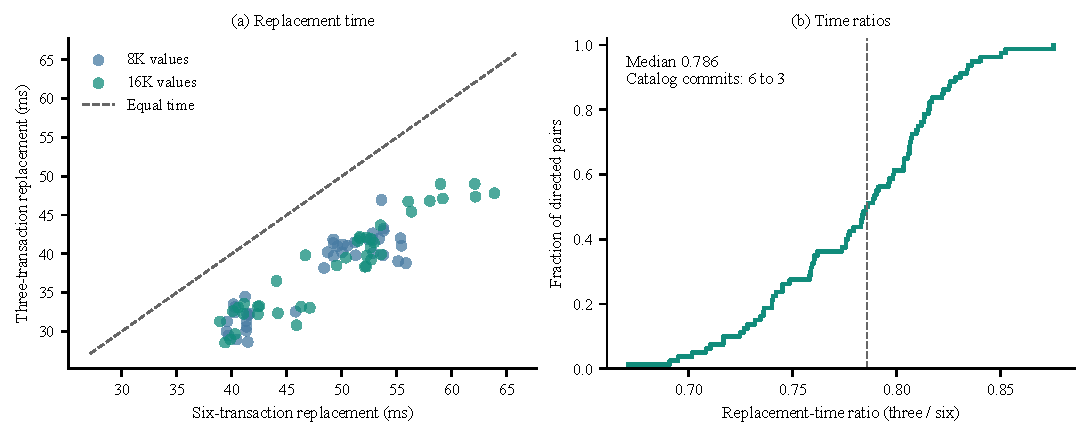
\includegraphics[width=.94\textwidth]{executor_cost.pdf}
\caption{Paired replacement costs.}
\label{fig:executor}
\end{figure*}
The equivalent count-table controller reduces median decision-boundary work from 90.1 to 47.1~$\mu$s in the alternating-order component diagnostic. Its median paired ratio is 0.523. All 2.88 million checked requests preserve the scanning implementation's decisions, counters, and recorded actions. In the final executions, controller initialization has a median of 8.69~ms and a maximum of 12.88~ms per eight-chunk instance. The additional conditional-count arrays have a median footprint of 0.363~MiB per instance.

The shared refined calibration completes 8,352 query-cost strata and 4,320 directed replacement observations. Its wall time is 400.9~s, including setup replacements. This commissioning expenditure is separate from the following steady-state policy measurements.


\subsection{RQ2: Selective migration and its service trade-off}
All 144 scheduled executions complete with 23,040,000 independently checked events, valid final arrays, and catalog integrity. All control policies share the revised executor; the separate diagnostic above measures the executor change. Tables~\ref{tab:newresults} and~\ref{tab:strata} retain every policy and both workload strata. Ratios are equal-weight geometric means, and brackets give paired-bootstrap 95\% intervals. Table~\ref{tab:newresults} uses Static as the denominator; rewriting includes target payloads and representation metadata.
\begin{table*}[!t]
\centering\small
\caption{Overall policy comparison.}
\label{tab:newresults}
\begin{tabular}{@{}lrrrrrr@{}}
\toprule
Policy & Service ratio & 95\% interval & Event p99 ratio & Migrations & Rewrite (MiB) & Control (\%) \\
\midrule
Static & 1.000 & -- & 1.000 & 0 & 0.000 & 0.00 \\
Shape-EWMA-BE & 1.054 & [1.025, 1.085] & 1.038 & 0 & 0.000 & 3.81 \\
Horizon-RePress & 0.998 & [0.934, 1.044] & 1.126 & 35 & 1.426 & 3.15 \\
Work-function & 1.007 & [0.971, 1.042] & 1.054 & 13 & 0.510 & 2.34 \\
Credit-RePress & 0.920 & [0.853, 0.986] & 1.264 & 155 & 5.595 & 5.16 \\
Risk-RePress & 0.947 & [0.884, 1.005] & 1.102 & 66 & 2.375 & 2.04 \\
\bottomrule
\end{tabular}
\end{table*}

\begin{table*}[!t]
\centering\small
\caption{Results by workload stratum.}
\label{tab:strata}
\begin{tabular}{@{}lrrrr@{}}\toprule
Stratum & Service / Static & Event p99 / Static & Service / Credit & Event p99 / Credit \\
\midrule
Continuous (18) & 1.023 [0.995, 1.052] & 1.140 [1.101, 1.184] & 1.026 [0.989, 1.066] & 0.825 [0.769, 0.880] \\
Persistent (6) & 0.750 [0.668, 0.830] & 0.997 [0.926, 1.053] & 1.039 [0.966, 1.110] & 1.033 [1.000, 1.068] \\
\bottomrule\end{tabular}
\end{table*}


Against Credit-RePress under identical calibrated inputs, Risk-RePress reduces migrations from 155 to 66 (57.4\%) and target rewriting from 5.595 to 2.375~MiB (57.5\%, computed from unrounded bytes). Its event-p99 ratio is 0.872 (95\% interval 0.816--0.928), with lower p99 in 20 of 24 instances. Its service-time ratio is 1.029 (0.995--1.065), placing the observed tail and rewrite reductions alongside the range of average-cost effects. Controller execution accounts for 2.04\% of Risk-RePress service and 5.16\% of Credit-RePress service. Figure~\ref{fig:comparison} plots service-time ratios in (a) and event-p99 ratios in (b), with paired-bootstrap 95\% intervals across 24 instances. Each row uses its named baseline as the denominator; ratios below one favor Risk-RePress. Event timing includes query, controller, and synchronous maintenance work, while admission evaluates calibrated query-path distributions. Work-function denotes the work-function-inspired baseline.

\FloatBarrier
\begin{figure*}[!t]
\centering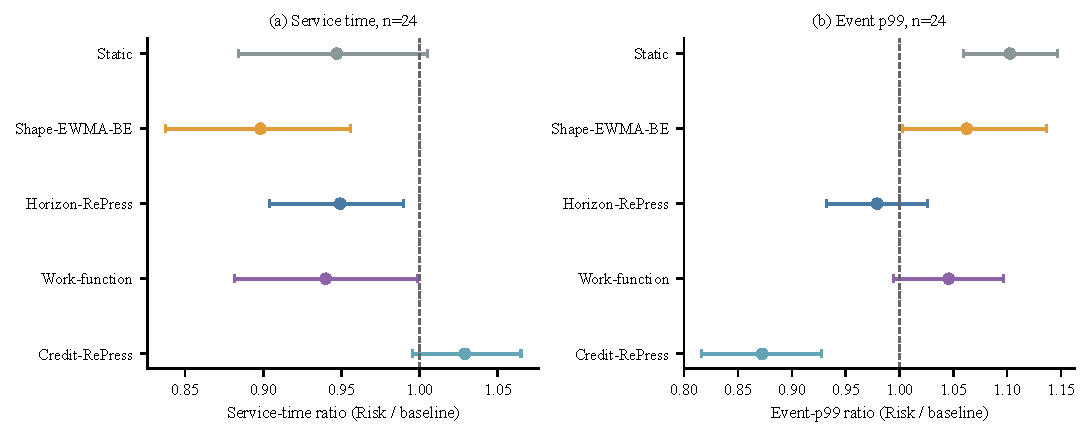
\includegraphics[width=.94\textwidth]{policy_comparison.pdf}
\caption{Service and event-tail comparisons.}
\label{fig:comparison}
\end{figure*}

The fixed-layout comparison addresses when adaptation pays. Under persistent shifts, Risk-RePress has a service ratio to Static of 0.750 (0.668--0.830), with a p99 ratio of 0.997 (0.926--1.053). Under continuous mixtures, the corresponding ratios are 1.023 (0.995--1.052) and 1.140 (1.101--1.184). A long point-heavy interval provides a different opportunity from repeated mixture changes. Panels (a,c) of Figure~\ref{fig:trajectories} show cumulative service relative to Static; panels (b,d) use Credit-RePress. Dotted lines in (c,d) identify the 20,000-query workload shift. Lines are geometric means; shading spans the 25th--75th percentiles across instances. Panels (a,b) use 18 continuous-mixture instances and (c,d) six persistent-shift instances. Risk and Credit denote Risk-RePress and Credit-RePress. Dashed horizontal lines mark parity; each column shares vertical limits. All instances contribute at every index; calibration and setup are accounted for separately. Across all 24 instances, the service ratio to Static is 0.947 (0.884--1.005) and the p99 ratio is 1.102 (1.059--1.146).

\begin{figure*}[!t]
\centering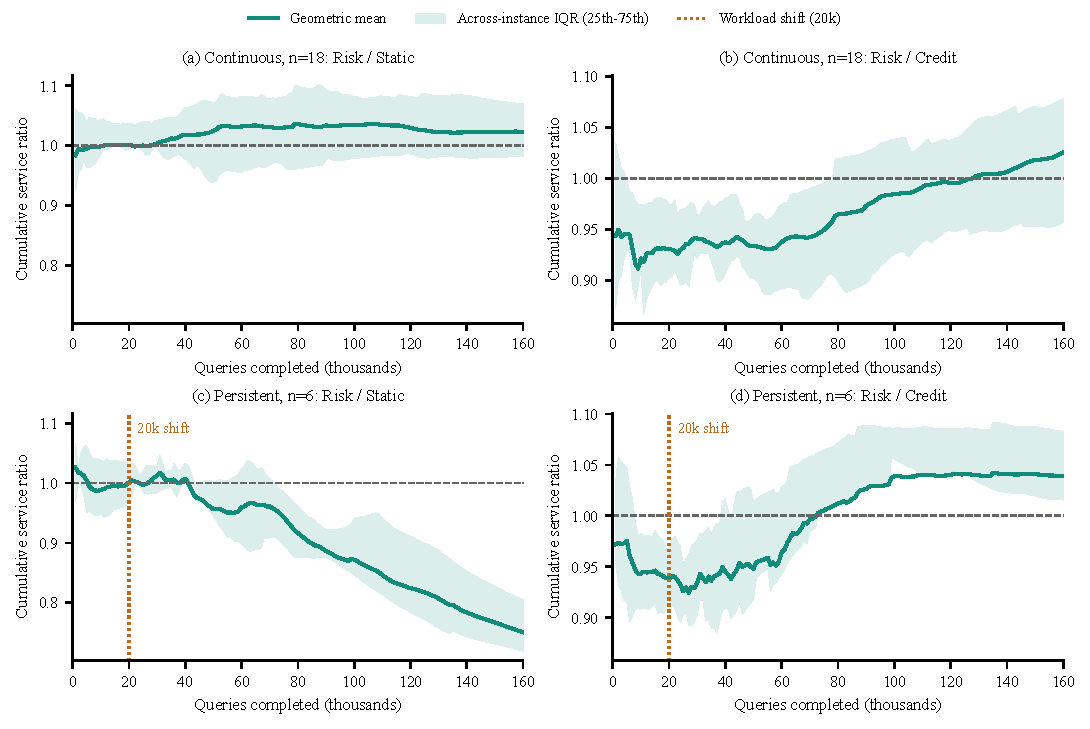
\includegraphics[width=.94\textwidth]{service_trajectories.pdf}
\caption{Cumulative service ratios.}
\label{fig:trajectories}
\end{figure*}

\subsection{Decision exposure and post-action opportunity}
\label{sec:mechanism}
Table~\ref{tab:decisions} partitions the 14,524 recorded decision boundaries; current-best and window-disagreement states share one logged category. At 13,473 boundaries the empirical tail test excludes at least one layout; in 7,620, the unconstrained mean-cost minimizer is excluded. These counts describe which choices the filter removes under the executed policy. At 364 of 1,205 confirmation- and cooldown-eligible price checks, the selected target's current evidence covers the forward-only threshold but remains below the installation-plus-return threshold. The controller produces 64 normal proposals and three repair proposals. One normal proposal is deferred by the byte budget; 63 normal replacements and three repairs execute. Credit-RePress and Horizon-RePress each record three budget deferrals, and every policy respects its payload cap. Joint policy comparisons quantify the resulting service and rewrite trade-offs.
\begin{table}[t]
\centering\small
\caption{Decision outcomes.}
\label{tab:decisions}
\begin{tabular}{@{}lr@{}}\toprule
Outcome & Boundaries \\
\midrule
Current best or window disagreement & 11,751 \\
Minimum gain test & 428 \\
Target confirmation & 1,137 \\
Evidence price & 1,141 \\
Proposed action & 67 \\
\midrule Total & 14,524 \\
\bottomrule\end{tabular}
\end{table}


For action $e$, let $I_e$ contain subsequent requests to its chunk through the query triggering the next replacement, or through the observed trace end. The triggering query of $e$ is served before that action. Post-action opportunity is
\begin{equation}
\widehat S_e=\sum_{t\in I_e}[\mu_{c_e}(r_e^-,x_t)-\mu_{c_e}(r_e^+,x_t)].
\label{eq:postaction}
\end{equation}
This is a counterfactual difference on the frozen calibration surface using the observed request sequence. We compare it with measured forward replacement time $M_e$ and unscaled calibrated price $P_e=m_{c_e}(r_e^-,r_e^+)+m_{c_e}(r_e^+,a_0)$. Admission applies the 1.25 margin to historical evidence in Eq.~\eqref{eq:admission}. Executed cost and calibrated price use distinct records: execution variability can place measured forward cost above the calibrated two-direction price. Episode coverage is evaluated at the last observed request; terminal episodes are right-censored at the trace end.
\begin{table*}[!t]
\centering\small
\caption{Post-action opportunity and cost.}
\label{tab:payback}
\begin{tabular}{@{}lrrrrr@{}}\toprule
Episode class & Episodes & $\widehat S_e\geq M_e$ & $\widehat S_e\geq P_e$ & Terminal & Median $\widehat S_e/M_e$ \\
\midrule
Continuous / normal & 20 & 14 & 12 & 17 & 1.56 \\
Continuous / repair & 3 & 0 & 0 & 3 & -16.53 \\
Persistent / normal & 43 & 40 & 41 & 43 & 6.30 \\
\bottomrule\end{tabular}
\end{table*}


In persistent shifts, 40 of 43 normal episodes have $\widehat S_e\geq M_e$, and 41 cover $P_e$; the median $\widehat S_e/M_e$ is 6.30. In continuous mixtures, 14 of 20 normal episodes cover $M_e$ and 12 cover $P_e$, with median ratio 1.56. Three normal episodes are closed by a return to the initial layout; one has modeled opportunity covering both executed replacements. The three repair episodes restore the empirically feasible reference and have negative mean-cost opportunity relative to the layouts they replace. Their measured costs remain in the service and rewrite totals. Model opportunity and realized service are complementary records: the latter also contains controller work and observed query-cost variation.

\subsection{Observed query tails and event tails}
Equation~\eqref{eq:feasible} concerns calibrated query-path distributions. The stable cohort contains 14,328 windows with 768 local requests under an unchanged layout and no migration at the decision boundary; 14,318 pass the model feasibility test. Table~\ref{tab:agreement} reports observed query and event p99 agreement within that model-feasible cohort; its last two columns count windows satisfying the 10\% paired tolerance. Agreement requires both the 256- and 768-query ratios to remain within 1.10. Paired ratios use identical requests from separately timed Static and Risk-RePress executions. The reference layout passes model feasibility by construction; separately timed queries still vary, and event timing also includes control work. Overlapping windows supply descriptive conditional counts; each workload instance remains the unit of the policy comparisons.
\begin{table}[t]
\centering\small
\caption{Tail agreement in stable windows.}
\label{tab:agreement}
\begin{tabular}{@{}lrrr@{}}\toprule
Layout & Model-feasible & Query p99 & Event p99 \\
\midrule
Reference & 11,851 & 6,084 & 3,967 \\
Adapted & 2,467 & 1,744 & 1,580 \\
\bottomrule\end{tabular}
\end{table}


The largest service ratio to Static occurs in the first group's 8K noisy-burst instance: 8.579 versus 7.410~s, with event p99 of 120.6 versus 99.2~$\mu$s. Its one migration costs 0.055~s, controller work costs 0.184~s, and query time differs by 0.931~s. These components preserve a concrete unfavorable instance alongside the aggregate comparisons.

\subsection{RQ3: Recovery across activation and retirement}
The new campaign contains 492 successful trials, summarized in Table~\ref{tab:recovery}. Controlled exceptions cover all 20 directed pairs over the original five layouts, both sizes, and ten software-visible stages. Additional checks exercise the 4,096-value layout in both directions against whole LZ4. Forty trials terminate the process directly. Twelve truncate the new payload after activation while the previous version remains retained. Reopening checks the active codec, exact values, query answers, catalog integrity, and repeated recovery.
\begin{table}[t]
\centering\small
\caption{Recovery test outcomes.}
\label{tab:recovery}
\begin{tabular}{@{}lrr@{}}\toprule
Trial class & Trials & Passed \\
\midrule
Controlled stage exceptions & 440 & 440 \\
Abrupt process exit & 40 & 40 \\
Post-activation payload truncation & 12 & 12 \\
\midrule Total & 492 & 492 \\
\bottomrule\end{tabular}
\end{table}

A separate abrupt-exit reproduction stops the original executor after old block metadata is deleted and before its cleanup transaction. Restart then raises a missing-metadata error while reconstructing the retained version. In the revised path, retirement has committed before this deletion stage; restart treats remaining old files as unreferenced garbage. The paired protocol trace and fault records bind this ordering to the executed implementation.
